\subsection{Experimental Setup}
Training is done in a two stage pipeline. The first stage is adaptive pretraining (PT) where a base pretrained English 13B GPT-2 model (\ref{base_model}) is continuously trained on a mixture composed of the new language and English. Then, the adapted checkpoint is instruction tuned (IT) on a collection of prompt completion pairs from the new language and English. For more information see appendix \ref{base_model},\ref{sec:dataset_details}

We categorize all evaluation tasks into 4 categories. {\textbf{Multiple Choice}, for this category we append each candidate answer to the prompt and pick the highest probability answer. \textbf{Open-ended Question Answering}, where we let the model generate an answer for each question, and report the average F1 score between the model output and the ground truth. \textbf{Summarization}, where we let the model generate a summary and report the average ROUGE-2 score between the model output and ground truth.
\textbf{Translation}, where we let the model generate translated text and report the BLEU score between the model output and the ground truth. When we report the score for each category, it is the averaged score of all the evaluation tasks that we classified into that category in appendix \ref{sec:evaluation}. 


% Whenever a bi-lingual training mixture is described below, the data is mixed such that the mixing ratio corresponds to the raw text file size ratio. Then the text is shuffled such that each sequence contains text from only one language, but the sequences are shuffled so that each batch will train on sequences from both languages.



\begin{table}[]
\centering
\caption{Each model is labeled by the language it is adapted for, followed by what style of training was done, The EN PT model is the base model for all following rows. PT stands for pretrained and IT stands for instruction tuned. Each column represents the average of all the benchmarks from a classified under a language and category, the constituent benchmarks can be found in appendix \ref{sec:evaluation}}
\label{tab:main_restult}
\begin{adjustbox}{max width=\textwidth}
\setlength{\tabcolsep}{2pt}
\begin{tabular}{ccccllllll}
\toprule
\multicolumn{1}{l}{} & English                   & \multicolumn{4}{c}{Hungarian}                                                                                            & \multicolumn{4}{c}{Thai}                                                                                                                     \\
\cmidrule(lr){2-2} \cmidrule(lr){3-6} \cmidrule(lr){7-10}
Tasks                & Multi-choice         & Multi-choice         & QA        & \multicolumn{1}{c}{Sum.} & \multicolumn{1}{c}{Trans.} & \multicolumn{1}{c}{Multi-choice} & \multicolumn{1}{c}{QA} & \multicolumn{1}{c}{Sum.} & \multicolumn{1}{c}{Trans.} \\
% \cmidrule(lr){2-2} \cmidrule(lr){3-6} \cmidrule(lr){7-10}
Metrics                & Acc. ($\uparrow$)         & Acc. ($\uparrow$)         & F1 ($\uparrow$)        & Rouge-2 ($\uparrow$)  & BLEU ($\uparrow$) & Acc. ($\uparrow$) & F1 ($\uparrow$)        & Rouge-2 ($\uparrow$)  & BLEU ($\uparrow$) \\
\midrule
Llama2-7B               &      59.2\%         &     43.9\%         &       4.3\%       &  \multicolumn{1}{c}{2.8}                                   &\multicolumn{1}{c}{}                                 & \multicolumn{1}{c}{47.1\%}                                  & \multicolumn{1}{c}{48.6\%}                                   & \multicolumn{1}{c}{\textbf{30.9}}                                   & \multicolumn{1}{c}{7.7} \\
XGLM-7.5B              &      51.9\%              &    42.8\%          &   \multicolumn{1}{c}{15.8\%}                                   &\multicolumn{1}{c}{0.4}                                 & \multicolumn{1}{c}{1.1}                                  & \multicolumn{1}{c}{46.8\%}                                   & \multicolumn{1}{c}{27.9\%}                                   & \multicolumn{1}{c}{0.0} & \multicolumn{1}{c}{0.2}\\
mt0-xxl              &       52.7\%        &       50.6\%       &    30.6\%          & \multicolumn{1}{c}{2.0}                                   &\multicolumn{1}{c}{\textbf{14.0}}                                 & \multicolumn{1}{c}{46.2\%}                                  & \multicolumn{1}{c}{\textbf{85.3\%}}                                   & \multicolumn{1}{c}{21.9}                                   & \multicolumn{1}{c}{0.9}                                 \\
PULI-GPT-3SX              &     33.5\%          &        43.2\%      &       35.9\%       & \multicolumn{1}{c}{3.1}                                   &\multicolumn{1}{c}{1.3}                                 & \multicolumn{1}{c}{-}                                  & \multicolumn{1}{c}{-}                                   & \multicolumn{1}{c}{-}                                   & \multicolumn{1}{c}{-}                                 \\
openthaigpt-7b-chat              &     \textbf{60.9\%}          &        -      &       -       & \multicolumn{1}{c}{-}                                   &\multicolumn{1}{c}{-}                                 & \multicolumn{1}{c}{43.7\%}                                  & \multicolumn{1}{c}{43.4\%}                                   & \multicolumn{1}{c}{26.5}                                   & \multicolumn{1}{c}{4.0}                                 \\
\midrule
EN PT                & 57.3\%              & 46.2\%              & 32.8\%              & \multicolumn{1}{c}{0.9}                                   &\multicolumn{1}{c}{1.9}                                 & \multicolumn{1}{c}{46.0\%}                                  & \multicolumn{1}{c}{14.4\%}                                   & \multicolumn{1}{c}{0.0}                                   & \multicolumn{1}{c}{0.2}                                 \\
EN PT + IT          & 57.3\%              & 45.9\%              & 34.4\%              & \multicolumn{1}{c}{1.3}         & \multicolumn{1}{c}{1.7}       &  \multicolumn{1}{c}{46.2\%}                                  & \multicolumn{1}{c}{16.1\%}                                   & \multicolumn{1}{c}{2.7}                                   & \multicolumn{1}{c}{0.0}                                \\
HU PT                & 55.3\%              & 44.9\%              & 48.5\%              & \multicolumn{1}{c}{3.7}                                  &  \multicolumn{1}{c}{7.7}                              & \multicolumn{1}{c}{-}                                  & \multicolumn{1}{c}{-}                                   & \multicolumn{1}{c}{-}                                   & \multicolumn{1}{c}{-}                                 \\
HU PT + IT           & 58.0\%              & \textbf{54.9}\%              & \textbf{64.3}\%              & \multicolumn{1}{c}{\textbf{9.2}}         & \multicolumn{1}{c}{6.1}       &  \multicolumn{1}{c}{-}                                & \multicolumn{1}{c}{-}                                    & \multicolumn{1}{c}{-}                                   & \multicolumn{1}{c}{-}                                 \\
TH PT                & 57.4\% & \multicolumn{1}{c}{-}   & \multicolumn{1}{c}{-}  &  \multicolumn{1}{c}{-}                                   & \multicolumn{1}{c}{-}                          & \multicolumn{1}{c}{48.4\%}  & \multicolumn{1}{c}{31.1\%}                                 &                          \multicolumn{1}{c}{11.4}       &                        \multicolumn{1}{c}{3.9}                                \\
TH PT + IT          & 56.4\% & \multicolumn{1}{c}{-}   & \multicolumn{1}{c}{-}   & \multicolumn{1}{c}{-}                                     & \multicolumn{1}{c}{-}                                   &   \multicolumn{1}{c}{\textbf{49.9\%}}                             &     \multicolumn{1}{c}{48.9\%}                              &                      \multicolumn{1}{c}{13.9}             &            \multicolumn{1}{c}{\textbf{12.5}}                     \\
\bottomrule         
\end{tabular}
\end{adjustbox}
\end{table}

\subsection{Main Results}\label{main_results}
We list all the results in table \ref{tab:main_restult}. The HU PT model is trained from EN PT with 50\% HU, 50\% EN data, and TH PT is similarly trained but with Thai data. The HU PT + IT model is trained from the HU PT checkpoint with 50\% HU, 50\% EN IT data. The TH PT + IT is similarly trained from the TH PT checkpoint with 50\% TH, 50\% EN IT data. The EN models trained on purely English data are used as baselines. We list out the dataset and training details in appendix \ref{sec:dataset_details}, \ref{sec:training_details}.

Table \ref{tab:main_restult} shows that with our proposed training recipe, the adapted models are able to maintain the performance on English benchmarks, and improve significantly on the benchmarks of the new languages. This confirms the effectiveness of replacing the tokens in the tokenizer and mixing training data to efficiently adapt a LLM to a new language. On top of this, the adapted models perform as well or better than the state of the art baseline models we have evaluated. 


\subsection{Ablation Studies}\label{ablation_study}

\subsubsection{Tokenizer}\label{tokenizer ablation}

\begin{wraptable}[5]{r}{0.36\textwidth}
\vspace{-56pt}
\captionof{table}{Performance of Hungarian model with different tokenizers. 
% The bilingual tokenizer is created using the method introduced in \ref{token replacement} 
}\label{tab:tokenizer_ablation}
\begin{adjustbox}{max width=\linewidth}
\begin{tabular}{ccc}
\toprule
\multicolumn{1}{l}{} & \multicolumn{1}{c}{GPT2} & Bilingual \\
\midrule
EN - Multi-choice    &   57.9\%                   & \textbf{58.0\%}   \\
HU- Multi-choice     &  50.8\%                    & \textbf{54.9\%}   \\
HU - QA              &       63.2\%                   & \textbf{64.3\%}   \\
HU - Sum.            &     7.9                    & \textbf{9.2}     \\
HU - Trans.          &  \textbf{8.8}                        & 6.1     \\
\bottomrule
\end{tabular}
\end{adjustbox}
\end{wraptable}

% To validate the token replacement method introduced in section \ref{token replacement}, an ablation study was run with both the original English tokenizer and the a tokenizer where 4k English tokens have been replaced by Hungarian. In this ablation we ran training for 30,000 steps with the hyperparameters in appendix \ref{pretraining hyperparameters} on dataset composed of 50\% Hungarian data and 50\% English data from section \ref{sec:dataset_details}. 
In this experiment, we evaluate models trained on identical data during both the continuous pretraining and IT stages. These models follow the same training recipe but use different tokenizers. Table \ref{tab:tokenizer_ablation} shows that \textbf{the model trained with the bilingual tokenizer performs as well or better than the model that uses the original tokenizer}, on both English and Hungarian tasks. While at the same time, the bilingual tokenizer has much better encoding efficiency as illustrated in Figure \ref{fig:fertility}. 


\subsubsection{Pretraining data mixture}\label{pretraining_data_mixture}
Given the same total amount of training data, we tested varying the percentage of English data (50\%, 25\% and 0\%) in the English/Hungarian bilingual data mixture. All training is run for 30k steps. We also compare this to training a pure Hungarian model using only Hungarian data \cite{Nemeskey:2020}, a Hungarian tokenizer, from scratch for 100k steps. All the training details can be found in appendix \ref{pretraining hyperparameters}.

\begin{wrapfigure}[16]{r}{7cm}
\vspace{-12pt}
\caption{Varying pretraining data mixtures. "EN" and "HU" models are monolingual models trained from scratch, while the other models are trained from the "EN" model with the labeled data mixture. }\label{fig:pretraining_mixture}
% \vspace{-6pt}
\begin{tikzpicture}
\begin{groupplot}[group style = {group size = 2 by 1, horizontal sep = 35pt}, width =\linewidth, height = 3.5cm]
    \nextgroupplot[
        ybar=0.0cm,
        bar width=5pt,
        width=0.55\linewidth, height=3.5cm,
        enlarge x limits=0.2,
        title=HU Eval Perplexity,
        title style={yshift=-1ex, font=\small},
	ymajorgrids,
        ylabel={Byte Perplexity $\downarrow$},
        ymin=0,
        xtick=data,
        ytick={0, 1, 2, 3},
        x tick label style={xshift=0.8ex,rotate=45,anchor=east,yshift=-2pt,font=\tiny},
        y label style={yshift=-3.5ex, font=\small},
        symbolic x coords = {EN, 50EN/50HU, 25EN/75HU, 0EN/100HU, HU},
        tickwidth         = 1pt,
        legend style={
            at={(1.1,-0.4)},
            anchor=north,
            legend columns=3,
            font=\tiny,
            /tikz/every even column/.append style={column sep=0.cm},
        },
    ]
        \addplot[black, fill=blue] coordinates { 
            (EN, 2.80)
            (50EN/50HU, 1.84)
            (25EN/75HU, 1.82)
            (0EN/100HU, 1.98)
            (HU, 2.05)
        };
    
    \nextgroupplot[
        ybar=0.0cm,
        bar width=5pt,
        width=0.55\linewidth, height=3.5cm,
        enlarge x limits=0.2,
        title=EN Multi-choice,
        title style={yshift=-1ex, font=\small},
	ymajorgrids,
        ylabel={Accuracy $\uparrow$},
        ymin=0,
        xtick=data,
        ytick={0, 30, 60, 90},
        x tick label style={xshift=0.8ex,rotate=45,anchor=east,yshift=-2pt,font=\tiny},
        y label style={yshift=-3.5ex, font=\small},
        symbolic x coords = {EN, 50EN/50HU, 25EN/75HU, 0EN/100HU, HU},
        tickwidth         = 1pt,
        legend style={
            at={(1.1,-0.4)},
            anchor=north,
            legend columns=3,
            font=\tiny,
            /tikz/every even column/.append style={column sep=0.cm},
        },
    ]
        \addplot[black, fill=blue] coordinates { 
            (EN, 55.9)
            (50EN/50HU, 52.5)
            (25EN/75HU, 54.0)
            (0EN/100HU, 37.2)
            (HU, 43.0)
        };
\end{groupplot}
\end{tikzpicture}
\end{wrapfigure} 


We summarize the comparison results in Figure \ref{fig:pretraining_mixture}. The first finding is that \textbf{it is effective to add in training data from the new language during pretraining}, because those models greatly outperformed the baseline English model. Second, \textbf{it is better to adapt a pretrained LLM than train a new one from scratch}, as the adapted checkpoint performs better on both languages, even though they are trained for one third as long. Third, when comparing the results from the models trained with and without English data mixed in, we can see that \textbf{mixing English data can mitigate the catastrophic forgetting on English and improve the model performance on Hungarian}. Note that there is no significant difference between mixing 50\% and 25\% of English data during training, which implies that adaptation is not sensitive to the exact mixture ratio as long as the original language and new language are included.

\subsubsection{IT data mixture}\label{it_data_mixture}

\begin{wrapfigure}[14]{r}{6.5cm}
\vspace{-16pt}
\caption{Model performance with different IT data mixture. ROUGE-2 score is reported for HU Sum, while accuracy and F1 scores are reported for the rest of the tasks.}\label{fig:IT_mixture}
\vspace{-4pt}
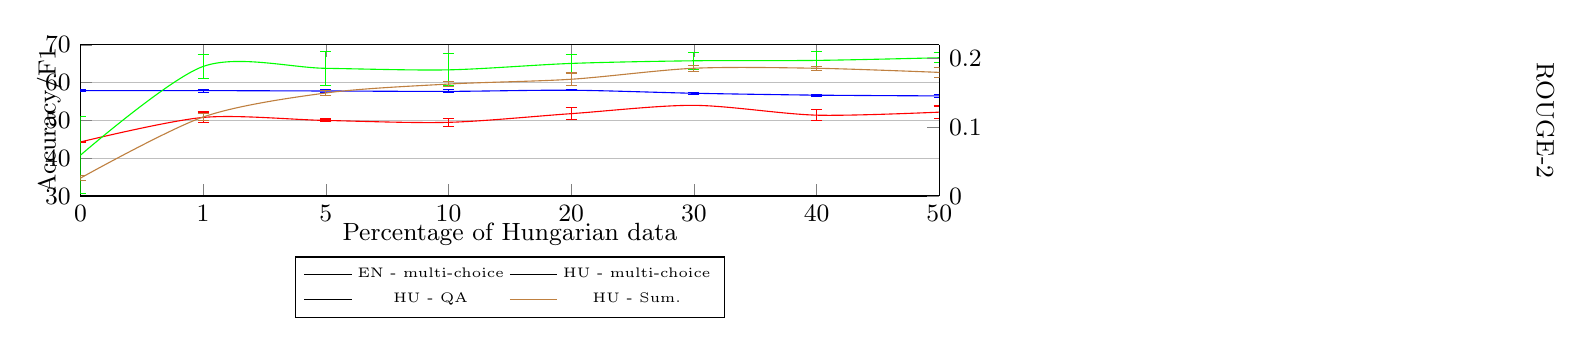
\begin{tikzpicture}
    \begin{axis}[
        xmin=0, xmax=50,
        ymin=30, ymax=70,
        xtick=data,
        symbolic x coords={0, 1, 5, 10, 20, 30, 40, 50},
        axis y line*=left,
        ytick={30,40,50,60,70},
        width=1.03\linewidth, height=3.5cm,
	ylabel=Accuracy/F1,
	ymajorgrids,
        y tick label style={font=\small},
        y label style={yshift=-3ex, font=\small},
	xlabel=Percentage of Hungarian data,
        x tick label style={font=\small},
        x label style={yshift=1.5ex, font=\small},
        legend style={
            at={(0.5,-0.4)},
            anchor=north,
            legend columns=2,
            font=\tiny,
            /tikz/every even column/.append style={column sep=0.cm},
        },
    ]
    \addplot [blue,smooth, error bars/.cd, y dir=both, y explicit] plot coordinates {
        (0, 57.9) +- (0.33, 0.33)
        (1, 57.9) +- (0.41, 0.41)
        (5, 57.8) +- (0.51, 0.51)
        (10,57.7) +- (0.38, 0.38)
        (20,58.0) +- (0.09, 0.09)
        (30,57.2) +- (0.25, 0.25)
        (40,56.7) +- (0.23, 0.23)
        (50,56.5) +- (0.34, 0.34)
    }; \label{plot_one}
    \addlegendentry{EN - multi-choice}

    \addplot[smooth,color=red, error bars/.cd, y dir=both, y explicit]
        plot coordinates {
        (0, 44.3) +- (0.10, 0.10)
        (1, 50.8) +- (1.45, 1.45)
        (5, 50.0) +- (0.39, 0.39)
        (10,49.5) +- (1.11, 1.11)
        (20,51.8) +- (1.54, 1.54)
        (30,54.0) +- (0.02, 0.02)
        (40,51.4) +- (1.40, 1.40)
        (50,52.2) +- (1.62, 1.62)
    }; \label{plot_two}
    \addlegendentry{HU - multi-choice}
    % \addlegendentry{LLaMA-30b}

    \addplot[smooth,color=green, error bars/.cd, y dir=both, y explicit]
        plot coordinates {
        (0, 40.8) +- (10.20, 10.20)
        (1, 64.3) +- (3.18, 3.18)
        (5, 63.8) +- (4.53, 4.53)
        (10,63.4) +- (4.25, 4.25)
        (20,65.1) +- (2.31, 2.31)
        (30,65.8) +- (2.26, 2.26)
        (40,65.9) +- (2.26, 2.26)
        (50,66.6) +- (1.29, 1.29)
    }; \label{plot_three}
    \addlegendentry{HU - QA}
    \end{axis}

    \begin{axis}[
      width=1.03\linewidth, height=3.5cm,
      axis y line*=right,
      axis x line=none,
      ymin=0, ymax=0.22,
      ylabel=ROUGE-2,
      y tick label style={font=\small},
      y label style={yshift=-45ex, rotate=180, font=\small},
      ytick={0,0.1,0.2},
      xtick=data,
      xmin=0, xmax=50,
      symbolic x coords={0, 1, 5, 10, 20, 30, 40, 50},
      legend style={
          at={(0.5,-0.4)},
          anchor=north,
          legend columns=2,
          font=\tiny,
          /tikz/every even column/.append style={column sep=0.cm},
      },
    ]
    \addlegendimage{/pgfplots/refstyle=plot_one}\addlegendentry{EN - multi-choice}
    \addlegendimage{/pgfplots/refstyle=plot_two}\addlegendentry{HU - multi-choice}
    \addlegendimage{/pgfplots/refstyle=plot_three}\addlegendentry{HU - QA}
    \addplot[smooth,brown, error bars/.cd, y dir=both, y explicit]
      coordinates{
        (0, 0.026) +- (0.0032, 0.0032)
        (1, 0.115) +- (0.0050, 0.0050)
        (5, 0.150) +- (0.0038, 0.0038)
        (10,0.163) +- (0.0038, 0.0038)
        (20,0.170) +- (0.0091, 0.0091)
        (30,0.186) +- (0.0041, 0.0041)
        (40,0.186) +- (0.0031, 0.0031)
        (50,0.180) +- (0.0076, 0.0076)
    }; 
    \addlegendentry{HU - Sum.}
    \end{axis}
\end{tikzpicture}
\end{wrapfigure} 

We run all instruction tuning experiments from the Hungarian pretrained model using 6 gigabytes of instruction tuning text data (2 billion tokens) and the same training settings. Each experiment is repeated 3 times with different random dataset samples. For more details on instruction tuning datasets or training settings see appendix \ref{english instruction tuning data}, \ref{hungarian instruction tuning data} and \ref{instruction tuning hyperparameters}

There is a lack of diverse high quality instruction tuning data in most languages besides English. Thus, we study the impact of the amount of IT data from the new language on the final model performance by varying the Hungarian instruction tuning data mixing rate from  0\% to 50\%. 
Figure \ref{fig:IT_mixture} shows that when no Hungarian instruction tuning data is included, the model undergoes catastrophic forgetting of Hungarian. 
However, the model performance on Hungarian improves as more Hungarian data is mixed in, with marginal returns after more than 1\% of the data is Hungarian. This indicates that a small amount of IT data from the new language gives most of the model performance on the new language.

% These models instruction tuned on purely English data become aligned, but when viewing the generations the models sometimes respond to Hungarian prompts in English even though they understood the question. But figure \ref{fig:IT_mixture}, also shows that even a small quantity of translated instruction data in the new language mixed with a large amount of English data, can be enough to avert catastrophic forgetting, and demonstrates the diminishing returns as more translated Hungarian Instruction data is included.

% \subsubsection{[Single-stage Training vs Two-stage Pretraining and IT}\label{Single-stage_Training_vs Two-stage_Pretraining_then_IT}
% TBD will we include?